\documentclass{article}

\usepackage{physics} % Handy shortcuts like \pdv, \dd and much more
\usepackage[top=2cm]{geometry} % smaller margins, can be adjusted if given arguments
\usepackage{siunitx} % the \si environment for units
\usepackage{mathtools} % The dcases environment, prettier than just cases
\usepackage{tikz} % For drawing picures
\usepackage{wrapfig} % Wrapping text around figures
\usepackage{enumitem} % Getting alphabetical enumerate


\title{Exercise 7 - TFY4345 Classical Mechanics}
\date{2020}

\begin{document}
    \maketitle
    \section{Inertia tensor}
    \begin{wrapfigure}{2}{0.3\textwidth}
        \includegraphics[width=0.3\textwidth]{figures/exercise_7_1_slab.pdf}
        \vspace{-2cm}
    \end{wrapfigure}
    A very thin uniform rectangular slab of mass $M$ has been placed in the $xyz$-coordinates system, such that the origin is in one of the slab corners, and the sides are along the $x$- and $y$-axes. The corresponding side lengths are $a$ and $b$. Since the slab is very thin, we can assume that $z=0$ throughout.
    \begin{enumerate}[label=(\alph*)]
        \item Evaluate the individual elements of the inertia tensor.
        \item Set $a = b$, and solve for the principal moments of inertia, and the corresponding principal axes.
    \end{enumerate}

    \section{Rotated tilted slab}
        \begin{wrapfigure}{r}{0.25\textwidth}
            \includegraphics[width=0.25\textwidth]{figures/exercise_7_2_slab.pdf}
        \end{wrapfigure}

        (Exam Aug. 2018)\\
        Consider the same thin slab. However, now it rotates around an axis parallel to its diagonal, with an angular velocity vector $\boldsymbol\omega$. As the axis of rotation has change, so has its principal axis. The principal axes $x_1$ and $x_2$ are parallel to the slab edges, as indicated in the figure, while the axis $x_3$ is perpendicular to the slab, and goes through its center. The side lengths of the slab are $a$ and $b$, with the principal moments of inertia

        \begin{equation*}
            I = 
            \begin{pmatrix}
                I_{1} & 0 & 0 \\
                0 & I_{2} & 0 \\
                0 & 0 & I_{3} \\
            \end{pmatrix}
            = M
            \begin{pmatrix}
                \frac{1}{12} a^2& 0 & 0 \\
                0 & \frac{1}{12} b^2 & 0 \\
                0 & 0 & \frac{1}{12} (a^2 + b^2)\\
            \end{pmatrix}
        \end{equation*}
        \begin{enumerate}[label=(\alph*)]
            \item Derive the angular momentum vector $\mathbf{L}$ of the slab, in terms of $a, b, M$ and $\omega$.
            \item What is the angle $\alpha$ between $\mathbf L$ and $\boldsymbol \omega$?
            \item What is the rotational kinetic energy $T$?
        \end{enumerate}

    \section{Cone rolling on a plane}
        \begin{figure*}
            \centering
            \includegraphics[width=0.7\textwidth]{figures/exercise_7_3_cone.pdf}
        \end{figure*} 
        (Exam Dec. 2016) \\
        We shall consider the motion of a solid cone that is rolling on the surface ($xy$-plane), without slipping. The center of mass of the cone is situated on the symmetry axis $x_3$, which goes through the center of the bottom of the cone. It is at a distance $\ell$ from the origin $O$. The height of the cone is $H$, and the radius of the bottom of the cone is $R$, and the cone half angle is $\alpha$. These are related by $R\cos(\alpha) = \sin(\alpha)  H$. The momentary line of contact between the cone and the $xy$-plane is the line $OA$, which is at an angle $\phi$ relative to the $x$-axis.
        \begin{enumerate}[label=(\alph*)]
            \item Calculate the velocity of the center of mass, $V_{CM}$ as a function of $\ell, \alpha$ and $\dv{t} \phi =\dot \phi$.
            \item Explain why the angular velocity vector $\boldsymbol \omega$ of the rolling cone is directed along the line $OA$, the line of contact between the cone and the $xy$-plane. Show that 
            \begin{equation*}
                \omega = |\boldsymbol \omega | = \frac{1}{\tan(\alpha)} \dot \phi
            \end{equation*}
            \item $x_3$ is one of the principal axis of rotations, what are the other? Remember that the coordinate transformation that takes $xyz$ into the principal axis $x_1x_2x_3$ is a rotation. Due to the symmetry of the cone, we have some freedom in choosing  the other two axis. Choose $x_1$ to be in the plane spanned by $\boldsymbol \omega$ and $x_3$, and find the components of $\boldsymbol \omega $ along the principal axes.
            \item The principal moment of inertia of the cone, for rotation around the point $O$ is
                \begin{equation*}
                    I = 
                    \begin{pmatrix}
                        I_{1} & 0 & 0 \\
                        0 & I_{2} & 0 \\
                        0 & 0 & I_{3} \\
                    \end{pmatrix}
                    = \frac{3}{20} M 
                    \begin{pmatrix}
                        R^2 + 4H^2& 0 & 0 \\
                        0 & R^2 + 4H^2& 0 \\
                        0 & 0 & 2R^2\\
                    \end{pmatrix}
                    ,
                \end{equation*}
                where $M$ is the mass of the cone. Calculate the kinetic energy of the cone as a function of $M, H, \alpha$ and $\dot \phi$.
        \end{enumerate}

\end{document}
